\part{The back end}\label{part:nstar}


\chapter{Introduction}\label{chap:nstar-abstract}

Assembly languages are the lowest level of humanly-possible programming there exists nowadays. They were used back in the days for very performance-critical tasks, or even just for fun, as there weren't many other programming languages available. Nowadays, with all the existing ones, most people have never used any assembly language.

Despite their apparent simplicity, and the small amount of work you need to put into creating assembly languages, those are in fact very hard to use. At that low level, there is no such thing as Java's exceptions keeping you from doing dumb things, Rust's linear types keeping you from leaking memory nor even Garbage Collectors. The nice things preventing you from having segfaults simply do not exist, and you are expected to either provide all those things yourself (creating a language runtime) or be very careful about what you are doing each time you write a single instruction (even a simple \texttt{mov} can have undesirable side-effects).

Doing dumb things is something that we must prevent directly when using the language. That way, we do not need to rely on external verification tools or debuggers, trying to know why a program segfaults at a specific point.
This is where a type system can become handy. Typed assembly languages are assembly languages augmented with simple yet powerful type system. Among the most famous typed assembly languages are TALx86~\cite{TALx86}, FunTAL~\cite{FunTAL} and DTAL~\cite{DTAL}.

TALx86 is basically NASM with a type system, targetting only the x86 architecture. DTAL is much more complicated and embeds a completely dependent type system. FunTAL is a more complex system than TALx86 (it is based on STAL~\cite{STAL}) and provides a fully-fledged type assembly language, almost entirely integrated inside a functional programming language.

\vspace{\baselineskip}

N*'s goal is to assist users with a simple but powerful type system, yet still allowing for low-level data manipulation.
But before even being a usable programming language, N* aims at being a compiler backend (much like for example LLVM), and is used that way in the Zilch project. Differences with other compiler backends are mostly the type-system, allowing the compilation of Zilch source code into type-safe instructions.

\vspace{\baselineskip}

Because N* supports compiling to multiple architectures, using different grammars, describing N* will at first be platform-agnostic, treating common aspects between all CPU architectures, and then will be divided into multiple categories, explaining in more details some features on a per-architecture basis\footnote{Note that the target executable format (ELF, PE, \ldots) is also considered as an architecture-specific thing, but should not influence N* much.}.

\section*{Small notes on the notation used in the next chapters}\label{sec:nstar-abstract-notation}

\begin{itemize}
  \item Kind inference
        \begin{itemize}
          \item $\Gamma$ is the typing context, containing every bindings from names to type variables;
          \item $\vdash^{K}$ is the kind inference judgement;
        \end{itemize}
  \item Type inference
        \begin{itemize}
          \item $\Xi$ is the context containing all bound labels, composed of two other contexts: $\Xi_{c}$ and $\Xi_{d}$. $\Xi_{c}$ contains all the labels defined in \texttt{code} sections, and $\Xi_{d}$ contains all the labels defined in \texttt{data} sections;
          \item $\chi$ is the current register-to-type mapping, and contains all known-to-be-bound registers.
                A register which is not present in this context means that either it has never been bound, or the value in it has been forgotten at some point;
          \item $\sigma$ is the current stack type;
          \item $\epsilon$ is the current continuation;
          \item $\vdash^{T}_{data}$ and $\vdash^{T}_{code}$ are the type inference judgements for expressions in their respective sections (\texttt{data} or \texttt{code}).
                $\vdash^{T}_{data}$ uses no context, whereas $\vdash^{T}_{code}$ uses all four of the defined contexts above (namely $\Xi$, $\chi$, $\sigma$ and $\epsilon$);
          \item $\Xi;\Gamma;\chi;\sigma;\epsilon\vdash^{I}instr\dashv\chi^\prime;\sigma^\prime;\epsilon^\prime$ denotes that the type inference of the instruction $instr$ in the current typing contexts $\Xi;\Gamma;\chi;\sigma;\epsilon$ yields a new typing context $\chi^\prime;\sigma^\prime;\epsilon^\prime$;
          \item $t1 \sim t2$ (and its counterpart $t1 \nsim t2$) respectively mean that $t1$ and $t2$ can be unified (or not);
        \end{itemize}
  \item Grammar
        \begin{figure}[H]
          \centering
          \scalebox{.5}{
            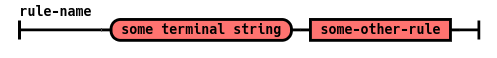
\includegraphics{grammar-template}
          }
        \end{figure}
        \begin{itemize}
          \item Normal rectangles describe other grammar rules (whose name is given in the shape);
          \item Rounded rectangles describe terminal nodes, that is invariant string pieces;
          \item The name of the grammar rule is given in the top-left corner of the diagram
                For a rule to match, it must be possible to go from one end to the other while staying on the black rails;
        \end{itemize}
\end{itemize}

\chapter{Non platform-specific features}\label{chap:nstar-common}

\section{Types}\label{sec:nstar-common-ts}

One of the differences between classical assembly languages and N* is its type system.
Compared to other higher level programming languages like Java, C++, etc, N* has a very simple yet powerful and expressive enough type system.

In programming, types are used mostly to prove at compile-time that a given program should behave well if it type-checks. While this works for more elaborated programming languages like Haskell, Idris, etc, most type systems aren't expressive enough to absolutely guarantee that everything will work at run-time (in fact, there is no possible way of doing this, because for example a memory allocation may fail, and this cannot be checked at compile-time). However, we can try to guarantee as much as possible.

N* doesn't try to solve this issue, because it would be really hard to target a dependently typed assembly language from a non-dependently typed programming language. But where all used assembly languages do not even consider types (only numbers, in fact), N* embeds a powerful type system used to remove the possibility of bugs (like incorrect structure addresses passed as a parameter function, or incoherent types in some instructions).

\subsection{Kinds}\label{subsec:nstar-common-ts-kinds}

Kinds (also known as types of types) mainly serve the purpose of indicating type sizes.
There are three type of kinds in N*:
\begin{itemize}
  \item Stack kind, denotating stack-like types, which can be safely offsetted
  \item Kinds whose size is abstracted away, useful to ask for any sized type
  \item Kinds whose size is already known
  \item Continuation kinds, for types that can be used as continuations
\end{itemize}
The grammar is given in Figure~\ref{fig:nstar-common-ts-kinds-syntax}.

\begin{figure}[htb]
  \centering
  \scalebox{.5}{
    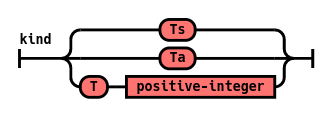
\includegraphics{nstar/types/kinds-syntax}
  }
  \caption{Grammar for kinds.}
  \label{fig:nstar-common-ts-kinds-syntax}
\end{figure}

\subsection{Integer types}\label{subsec:nstar-common-ts-integer}

Numbers are the building block of any assembly language. Most of data manipulated is manipulated as numbers, e.g.\ addresses, characters, strings, enumerations, etc.
This is not the case in N*, where ``integer''  only really means ``number''.
The syntax for the types of integers is given in Figure~\ref{fig:nstar-common-ts-integer-syntax}.

\begin{figure}[htb]
  \centering
  \scalebox{.5}{
    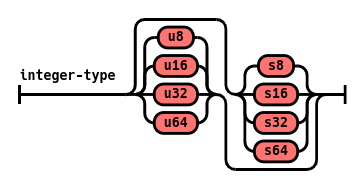
\includegraphics{nstar/types/integers-syntax}
  }
  \caption{Grammar for integer types.}
  \label{fig:nstar-common-ts-integer-syntax}
\end{figure}

Integers have two varying parameters: their sign and sizes.
According to the sign (i.e.\ signed or unsigned), some operations may not perform the same (for example \texttt{mul} does not behave the same).
The size is nothing more than the number of bits occupied by the integer (in N*, those are restricted to powers of 2 between $8$ and $64$ included).
Most operations should perform the same no matter the integer size, however it is recommended to search in the target architecture manual for further reference.

Kinds of integers are written under the form of inference rules in Figure~\ref{fig:nstar-common-ts-integer-kindrules}.

\begin{figure}[htb]
  \centering

  \begin{prooftree}
    \infer0{\Gamma\vdash^K$ u64 : T8$}
  \end{prooftree}
  \hspace{3em}
  \begin{prooftree}
    \infer0{\Gamma\vdash^K$ s64 : T8$}
  \end{prooftree}
  \hspace{3em}
  \begin{prooftree}
    \infer0{\Gamma\vdash^K$ u32 : T4$}
  \end{prooftree}
  \hspace{3em}
  \begin{prooftree}
    \infer0{\Gamma\vdash^K$ s32 : T4$}
  \end{prooftree}
  \\\vspace{\baselineskip}
  \begin{prooftree}
    \infer0{\Gamma\vdash^K$ u16 : T2$}
  \end{prooftree}
  \hspace{3em}
  \begin{prooftree}
    \infer0{\Gamma\vdash^K$ s16 : T2$}
  \end{prooftree}
  \hspace{3em}
  \begin{prooftree}
    \infer0{\Gamma\vdash^K$ u8 : T1$}
  \end{prooftree}
  \hspace{3em}
  \begin{prooftree}
    \infer0{\Gamma\vdash^K$ s8 : T1$}
  \end{prooftree}

  \caption{Kind inference rules for integers.}
  \label{fig:nstar-common-ts-integer-kindrules}
\end{figure}

\subsection{Other atomic types}\label{subsec:nstar-common-ts-otheratomic}

There are two other atomic types that we did not talk about, but refered to in the introduction of the type system: characters and pointers. Their respective syntax is given in Figure~\ref{fig:nstar-common-ts-atomic-syntax}.

\begin{figure}[htb]
  \centering
  \scalebox{.5}{
    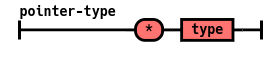
\includegraphics{nstar/types/ptr-syntax}
  } \\
  \scalebox{.5}{
    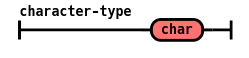
\includegraphics{nstar/types/char-syntax}
  }
  \caption{Grammar for character and pointer types}
  \label{fig:nstar-common-ts-atomic-syntax}
\end{figure}

In all assembly languages, characters are merely syntactic sugar for their ASCII code. This is how their are put in the machine code anyway, so it is not a huge problem (it might even not be at all).

Pointers, on the other hand, are unabstracted memory addresses.
In N*, there are two types of pointers: data pointers and stack pointers.
Stack pointers are covered in Subsection~\ref{subsec:nstar-common-ts-stack}~``\nameref{subsec:nstar-common-ts-stack}''.
Data pointers simply represent an address where we know (or not, see the Subsection~\ref{subsec:nstar-common-unsafe-derefliteraladdr}~``\nameref{subsec:nstar-common-unsafe-derefliteraladdr}'') that there is a value of the given pointed type.

Kind inference is given in Figure~\ref{fig:nstar-common-ts-atomic-kindrules}.

They support two common operations: offsetting (see the Subsection~\ref{subsec:nstar-common-unsafe-ptroffset}~``\nameref{subsec:nstar-common-unsafe-ptroffset}'') and dereferencing (taking the value pointed by the pointer).
Dereferencing is considered a safe operation, unless trying to on a literal address.
There is no notion of ``null'' pointers, like \texttt{NULL} in C.
However, it is possible to use the literal \texttt{\$0} (which represents a pointer to the address $0$).

\begin{figure}[htb]
  \centering
  \begin{prooftree}
    \infer0{\Gamma\vdash^K$ char : T1$}
  \end{prooftree}
  \hspace{3em}
  \begin{prooftree}
    \hypo{\Gamma\vdash^K$ t : Ta$}
    \infer1[64-bits pointers]{\Gamma\vdash^K$ *t : T8$}
  \end{prooftree}
  \hspace{3em}
  \begin{prooftree}
    \hypo{\Gamma\vdash^K$ t : Ta$}
    \infer1[32-bits pointers]{\Gamma\vdash^K$ *t : T4$}
  \end{prooftree}

  \caption{Kind inference rules for other atomic types.}
  \label{fig:nstar-common-ts-atomic-kindrules}
\end{figure}

\subsection{Context types}\label{subsec:nstar-common-ts-records}

Record types (or contexts) are mappings from registers to types, which also hold information about the current stack, as well as the return continuation.
They are used to indicate that a register is bound to a value of a given type at a certain point in the program.
The grammar is described in Figure~\ref{fig:nstar-common-ts-records-syntax}.

\begin{figure}[htb]
  \centering
  \scalebox{.5}{
    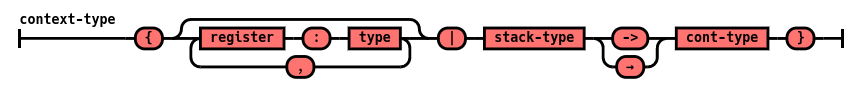
\includegraphics{nstar/types/records-syntax}
  }
  \\
  \scalebox{.5}{
    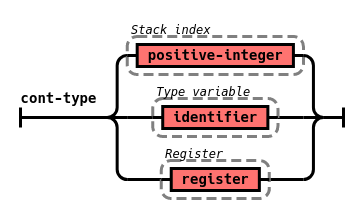
\includegraphics{nstar/types/continuation-syntax}
  }
  \caption{Grammar for context and continuation types.}
  \label{fig:nstar-common-ts-records-syntax}
\end{figure}

\begin{figure}[htb]
  \centering

  \begin{prooftree}
    \hypo{\Gamma\vdash^K\hat{\chi}}
    \hypo{\Gamma\vdash^K$ s : Ts$}
    \hypo{\Gamma\vdash^K$ e : Tc$}
    \infer3{\Gamma\vdash^K$\{ $\hat{\chi}$ | s $\to$ e \} : Ta$}
  \end{prooftree}

  \caption{Type inference rules for record types.}
  \label{fig:nstar-common-ts-records-typerules}
\end{figure}

Context types are used to represent data contexts where any mapping is some sort of a proof that some data of some type is accessible through some register.

\vspace{\baselineskip}

\textbf{Note:} In the context of label types (and more generally code addresses), a context type is augmented by a \texttt{forall} generic type variable binder.
The grammar is described in Figure~\ref{fig:nstar-common-ts-label-types-syntax}.
The type variable binder is used to abstract away some details of the type through an opaque variable specialized at the call site.

\begin{figure}[htb]
  \centering
  \scalebox{.5}{
    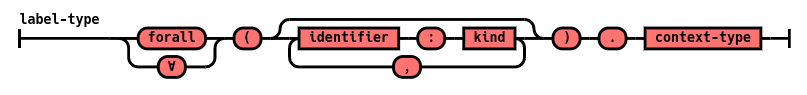
\includegraphics{nstar/types/label-syntax}
  }
  \caption{Grammar for label context types.}
  \label{fig:nstar-common-ts-label-types-syntax}
\end{figure}

\begin{figure}[htb]
  \centering

  \begin{prooftree}
    \hypo{\Gamma,\hat{v}\vdash^K$ ctx : Ta$}
    \infer1{\Gamma\vdash^K\forall$($\hat{v}$).ctx : T8$}
  \end{prooftree}

  \caption{Type inference rules for label context types.}
  \label{fig:nstar-common-ts-label-types-typerules}
\end{figure}

The example code given in Listing~\ref{lst:nstar-common-ts-records-stackmask} shows a use for type variables.
The stack is abstracted away, meaning that we can call this function from anywhere, given any stack (as long as it is \texttt{call}ed, or \texttt{jmp}ed to from a \texttt{call}ed function).
The type variable \texttt{s} is specialized at the call site.

\begin{listing}[htb]
  \centering
  \begin{minipage}{0.90\textwidth}
    \begin{minted}[]{\nstarlexer}
      label: forall(s: Ts, e: Tc). { %r0: forall(). {| s -> e } | s -> %r0 }
          ret
    \end{minted}
  \end{minipage}
  \caption{Stack masking using a type variable binder.}
  \label{lst:nstar-common-ts-records-stackmask}
\end{listing}

\subsection{Stack types}\label{subsec:nstar-common-ts-stack}

There is one stack type in N*: the stack constructor \texttt{::}.
Note that there is no ``empty stack'' type as would be the case with e.g.\ lists in Haskell.
The reason is that it forces the developer to abstract the stack to be able to have a ``stack tail'' (the part of the stack on the right of the stack constructor \texttt{::}) at some point.\footnote{It also serves the purpose to ensure that we cannot construct a stack from nothing, and that it should always be given to us, to e.g.\ the \texttt{main} function.}
An example is given in Listing~\ref{lst:nstar-common-ts-records-stackmask}.

The grammar for stack types is given in Figure~\ref{fig:nstar-common-ts-stack-types-syntax}.

Inference rules for kinds of stack types are written in Figure~\ref{fig:nstar-common-ts-stack-types-kindrules}

\begin{figure}[htb]
  \centering
  \scalebox{.5}{
    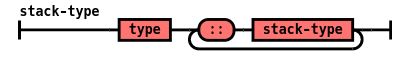
\includegraphics{nstar/types/stack-cons-syntax}
  }
  \caption{Grammar for stack types.}
  \label{fig:nstar-common-ts-stack-types-syntax}
\end{figure}

\begin{figure}[htb]
  \centering

  \begin{prooftree}
    \hypo{$n : $\mathbb{N}$ $}
    \hypo{\Gamma\vdash^K$ t : Tn$}
    \hypo{\Gamma\vdash^K$ s : Ts$}
    \infer3{\Gamma\vdash^K$ t :: s : Ts$}
  \end{prooftree}

  \caption{Kind inference rules for stack types}
  \label{fig:nstar-common-ts-stack-types-kindrules}
\end{figure}

\subsection{Structure types}\label{subsec:nstar-common-ts-structs}

Structure types are packed sets of unnamed types (compared to context types, each field does not have a name, only a type) that can be indexed from a pointer only to a full field (so if you have two \texttt{u64}s, you can only offset to $0$ and $8$, respectively for the first and second field).

Grammar is described in Figure~\ref{fig:nstar-common-ts-structs-syntax} and kind inference rules are given in Figure~\ref{fig:nstar-common-ts-structs-kindrules}.

Structures take as much space as all their fields, thus can mainly be put on the stack (unless being less than 8 bytes, which is the upper limit for register sizes in current architectures).

\begin{figure}[htb]
  \centering
  \scalebox{.5}{
    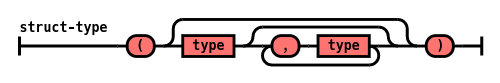
\includegraphics{nstar/types/struct-syntax}
  }

  \caption{Grammar for structure types.}
  \label{fig:nstar-common-ts-structs-syntax}
\end{figure}

\begin{figure}[H]
  \centering
  \begin{prooftree}
    \hypo{$n$_0$, n$_1$, $\ldots$, n$_p$ : $\mathbb{N}}
    \hypo{\Gamma\vdash^K$ t$_0$ : Tn$_0$, t$_1$ : Tn$_1$, $\ldots$, t$_p$ : Tn$_p}
    \hypo{$m = $\sum_{i = 0}^{p}{n_i}}
    \infer3{\Gamma\vdash^K$ (t$_0$, t$_1$, $\ldots$, t$_p$) : Tm$}
  \end{prooftree}

  \caption{Kind inference rule for structures.}
  \label{fig:nstar-common-ts-structs-kindrules}
\end{figure}

\subsection{Union types}\label{subsec:nstar-common-ts-unions}

Union types simply are overlapping data bits, which can be given meaning depending on what type you decide to access.
Grammar for union types is given in Figure~\ref{fig:nstar-common-ts-unions-syntax}.

\begin{figure}[htb]
  \centering
  \scalebox{.5}{
    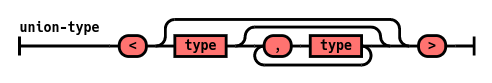
\includegraphics{nstar/types/union-syntax}
  }

  \caption{Grammar for union types.}
  \label{fig:nstar-common-ts-unions-syntax}
\end{figure}

Unions are sized depending on the types they unite: their sizes will be the maximum of all the sizes of all the components.
This is more clear in the kind inference rule given in Figure~\ref{fig:nstar-common-ts-unions-kindrules}.

\begin{figure}[H]
  \centering

  \begin{prooftree}
    \hypo{$n$_0$, n$_1$, $\ldots$, n$_p$ : $\mathbb{N}}
    \hypo{\Gamma\vdash^K$ t$_0$ : Tn$_0$, t$_1$ : Tn$_1$, $\ldots$, t$_p$ : Tn$_p}
    \hypo{$m = $\max_{i = 0}^{p}{n_i}}
    \infer3{\Gamma\vdash^K$ $\langle$t$_0$, t$_1$, $\ldots$, t$_p\rangle$ : Tm$}
  \end{prooftree}

  \caption{Kind inference rules for union types.}
  \label{fig:nstar-common-ts-unions-kindrules}
\end{figure}

Note that unlike structure types, you will most likely be storing union types in registers, unless working with very big unions.
Also, accessing a union's field is considered an unsafe operation, but this will be more detailed in another section on expressions.

\section{Expressions}\label{sec:nstar-common-expressions}

There are four types of expressions in N*: immediate values, data labels, registers and pointer offsets.
All of these can be used as the source operand of the \texttt{mov} instruction.

\subsection{Immediate values}\label{subsec:nstar-common-expressions-immediate}

Immediate values are also known as ``hardcoded values''.
These are values that you can directly read in the source file, and which do not come from e.g.\ registers.
Grammar and inference rules are given respectively in Figure~\ref{fig:nstar-common-expressions-immediate-grammar} and Figure~\ref{fig:nstar-common-expressions-immediate-typerules}.

\begin{figure}[H]
  \centering
  \scalebox{.5}{
    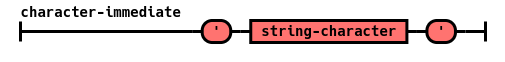
\includegraphics{nstar/exprs/imm-char-grammar}
  }
  \\
  \scalebox{.5}{
    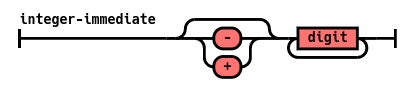
\includegraphics{nstar/exprs/imm-int-grammar}
  }
  \caption{Grammar for immediate values in N*.}
  \label{fig:nstar-common-expressions-immediate-grammar}
\end{figure}

\begin{figure}[H]
  \centering

  \begin{prooftree}
    \hypo{$c is a character immediate$}
    \infer1{\Xi;\Gamma;\chi;\sigma;\epsilon\vdash^T_{code}$ c : char$}
  \end{prooftree}
  \\\vspace{\baselineskip}
  \begin{prooftree}
    \hypo{$i is an unsigned integer immediate$}
    \hypo{$t $\in\{$ u8, u16, u32, u64 $\}}
    \infer2{\Xi;\Gamma;\chi;\sigma;\epsilon\vdash^T_{code}$ i : t$}
  \end{prooftree}
  \\\vspace{\baselineskip}
  \begin{prooftree}
    \hypo{$i is a signed integer immediate$}
    \hypo{$t $\in\{$ s8, s16, s32, s64 $\}}
    \infer2{\Xi;\Gamma;\chi;\sigma;\epsilon\vdash^T_{code}$ i : t$}
  \end{prooftree}

  \caption{Type inference rules for immediate values in N*.}
  \label{fig:nstar-common-expressions-immediate-typerules}
\end{figure}

\subsection{Labels}\label{subsec:nstar-common-expressions-labels}

\subsubsection{Data labels}\label{subsubsec:nstar-common-expressions-labels-data}

Data labels are pointers to some piece of data (may it even be an array).
They can be dereferenced and offset using the constructs given in N*.
Grammar and inference rules are given respectively in Figure~\ref{fig:nstar-common-expressions-labels-data-grammar} and Figure~\ref{fig:nstar-common-expressions-labels-data-typerules}.

\begin{figure}[H]
  \centering

  \scalebox{.5}{
    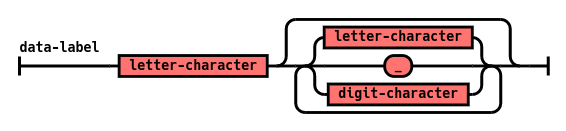
\includegraphics{nstar/exprs/label-expr-grammar}
  }
  \caption{Grammar for data labels in N*.}
  \label{fig:nstar-common-expressions-labels-data-grammar}
\end{figure}

\begin{figure}[H]
  \centering

  \begin{prooftree}
    \hypo{$l : t $\in\Xi_d}
    \infer1{\Xi;\Gamma;\chi;\sigma;\epsilon\vdash^T_{code}$ l : *t$}
  \end{prooftree}

  \caption{Type inference rules for data labels in N*.}
  \label{fig:nstar-common-expressions-labels-data-typerules}
\end{figure}

\subsubsection{Code labels}\label{subsubsec:nstar-common-expressions-labels-code}

Code labels are pointers to some piece of executable instructions.
Unlike data labels, they cannot be dereferenced or offset, but are instead automatically boxed.
Grammar and inference rules are given respectively in Figure~\ref{fig:nstar-common-expressions-labels-code-grammar} and Figure~\ref{fig:nstar-common-expressions-labels-code-typerules}.

\begin{figure}[H]
  \centering

  \scalebox{.5}{
    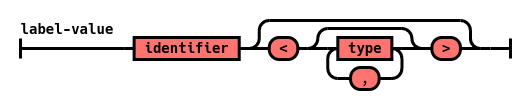
\includegraphics{nstar/exprs/label-value-grammar}
  }
  \caption{Grammar for code labels in N*.}
  \label{fig:nstar-common-expressions-labels-code-grammar}
\end{figure}

\begin{figure}[H]
  \centering

  \begin{prooftree}
    \hypo{$l : $\forall$($\vec{v}$).ctx $\in\Xi_c}
    \hypo{\Gamma\vdash^K$ s$_1$ : k$_1$, s$_2$ : k$_2$, \ldots, s$_p$ : k$_p}
    \infer[no rule, rule margin=1.0ex]2{\vec{s}$ = $\{$ s$_1$ : k$_1$, s$_2$ : k$_2$, \ldots, s$_p$ : k$_p$ $\}$\hspace{1.5em}$%
                                        \vec{s}\sim\vec{v}}
    \infer1{\Xi;\Gamma;\chi;\sigma;\epsilon\vdash^T_{code}$ l<$\vec{s}$> : $\forall$().ctx$}
  \end{prooftree}

  \caption{Type inference rules for code labels in N*.}
  \label{fig:nstar-common-expressions-labels-code-typerules}
\end{figure}

\subsection{Registers}\label{subsec:nstar-common-expressions-registers}

Registers in N* are abstracted away from the target architectures.
Instead of manipulating registers \texttt{\%eax} or \texttt{\%rsp} or \texttt{\$a2}, which all are platform-specific, there are 6 general purpose registers in N*, named \texttt{r0} to \texttt{r5}.
They can be 4 to 8 bytes large depending on the target architecture mappings.

Grammar for all those registers is given in Figure~\ref{fig:nstar-common-expressions-registers-grammar} and inference rules are given in Figure~\ref{fig:nstar-common-expressions-registers-typerules}.

\begin{figure}[htb]
  \centering

  \scalebox{.5}{
    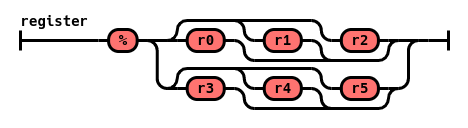
\includegraphics{nstar/exprs/register-grammar}
  }

  \caption{Grammar for registers in N*.}
  \label{fig:nstar-common-expressions-registers-grammar}
\end{figure}

\begin{figure}[htb]
  \centering

  \begin{prooftree}
    \infer0{\Xi;\Gamma;\chi$, r : t$;\sigma;\epsilon\vdash^T_{code}$ r : t$}
  \end{prooftree}

  \caption{Type inference rules for registers in N*}
  \label{fig:nstar-common-expressions-registers-typerules}
\end{figure}

\subsection{Pointer offsets}\label{fig:nstar-common-expressions-pointeroffsets}

Pointer offsets allow accessing data that may be located relative to a given memory address.
Grammar for pointer offsets is given in Figure~\ref{fig:nstar-common-expressions-pointeroffsets-grammar} and type inference rules are given in Figure~\ref{fig:nstar-common-expressions-pointeroffsets-typerules}.

\begin{figure}[H]
  \centering

  \scalebox{.5}{
    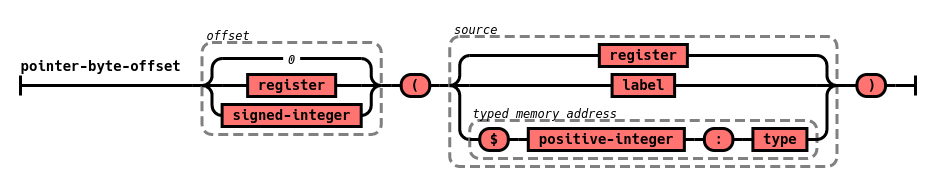
\includegraphics{nstar/exprs/pointer-byte-offset-grammar}
  }
  \\
  \scalebox{.5}{
    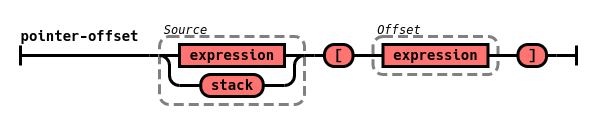
\includegraphics{nstar/exprs/pointer-offset-grammar}
  }

  \caption{Grammar for pointer offsets.}
  \label{fig:nstar-common-expressions-pointeroffsets-grammar}
\end{figure}

\begin{figure}[H]
  \centering

  \begin{prooftree}
    \hypo{\Gamma\vdash^K$ t : k$}
    \hypo{\Xi;\Gamma;\chi;\sigma;\epsilon\vdash^T_{code}$ p : *t$}
    \hypo{\Xi;\Gamma;\chi;\sigma;\epsilon\vdash^T_{code}$ o : s64$}
    \infer3[raw pointer byte offset]{\Xi;\Gamma;\chi;\sigma;\epsilon\vdash^T_{code}$ o(p) : *t$}
  \end{prooftree}
  \\\vspace{\baselineskip}
  \begin{prooftree}
    \hypo{\Gamma\vdash^K$ t : k$}
    \hypo{\Xi;\Gamma;\chi;\sigma;\epsilon\vdash^T_{code}$ p : *t$}
    \hypo{\Xi;\Gamma;\chi;\sigma;\epsilon\vdash^T_{code}$ o : s64$}
    \infer3[raw pointer base offset]{\Xi;\Gamma;\chi;\sigma;\epsilon\vdash^T_{code}$ p[o] : *t$}
  \end{prooftree}
  \\\vspace{\baselineskip}
  \begin{prooftree}
    \hypo{\Gamma\vdash^K$ t$_1$ : Tn$_0$, t$_2$ : Tn$_1$, \ldots, t$_m$ : Tn$_{m-1}}
    \infer[no rule, rule margin=1.0ex]1{$n$_0$, n$_1$, \ldots, n$_p\in\mathbb{N}$\hspace{1.5em}$%
                                        \Xi;\Gamma;\chi;\sigma;\epsilon\vdash^T_{code}$ p : *(t$_1$, t$_2$, \ldots, t$_m$)$}
    \infer1[structure pointer offset]{\Xi;\Gamma;\chi;\sigma;\epsilon\vdash^T_{code}$ p[n$_i$] : *t$_{i-1}}
  \end{prooftree}

  \caption{Type inference rules for pointer offsets.}
  \label{fig:nstar-common-expressions-pointeroffsets-typerules}
\end{figure}

Although offsetting a pointer works with any expression as the offset (as long as it is a signed integer), if the offset is a register, it is considered an unsafe operation\footnote{See Section~\ref{subsec:nstar-common-unsafe-ptroffsetreg}~``\nameref{subsec:nstar-common-unsafe-ptroffsetreg}''}.

\section{File sections}\label{sec:nstar-common-sections}

Sections in N* serve the exact same purpose as in other assembly languages. They divide a file into multiple parts depending on what the semantics of the current section is supposed to be (code, data, etc).
Section names obviously differ from one target format to another. As an example, the ``\texttt{.rela.dyn}'' section from the ELF format may not exist in the PE format.

N* tries to unify target formats section names (simplifying targetting N* as a compiler backend) by having a fixed set of section names, all with different meanings. While you can put anything anywhere in classical assembly languages, this is not the case in N*.

Sections in N* can be named ``\texttt{data}'', ``\texttt{code}'', ``\texttt{rodata}'', ``\texttt{udata}'' or ``\texttt{extern}''. Each of them has defined semantics as described below.

\subsection{The \texttt{code} section}\label{subsec:nstar-common-sections-code}

The \texttt{code} section is the section containing all executable instructions (basically, as the name implies, code).
Its syntax is defined in Figure~\ref{fig:nstar-common-sections-code-grammar}.

Each label is assigned a type, describing the context needed to branch to it.
If a label has the type \texttt{\{reg:s64\}} then there needs to be the register \texttt{reg} bound to a value of type \texttt{s64} in the current context, in order to branch to it.
However, some restrictions apply to labels in order to make the type-checking meaningful (or at least handle some aspects that cannot be handled with types only). See more about that in Section~\ref{sec:nstar-common-bs-restrictions}~``\nameref{sec:nstar-common-bs-restrictions}''.

\begin{figure}[htb]
  \centering
  \scalebox{.5}{
    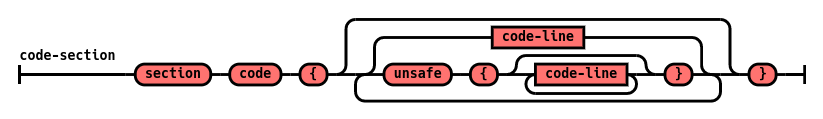
\includegraphics{nstar/sections/code-1}
  }
  \\
  \scalebox{.5}{
    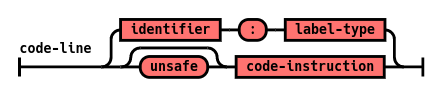
\includegraphics{nstar/sections/code-2}
  }
  \\
  \scalebox{.5}{
     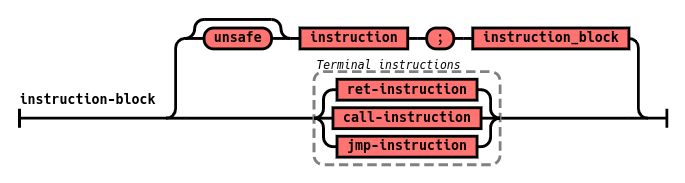
\includegraphics{nstar/sections/code-3}
  }

  \caption{Grammar for \texttt{code} sections.}
  \label{fig:nstar-common-sections-code-grammar}
\end{figure}

Every assembly instruction makes the current context vary in some way, either by binding registers, forgetting about some bindings, changing register types, or some other way. The current context is just a record keeping track of the currently bound registers, along with the data type they contain.
More on that in sections about instructions\footnote{Instructions are platform-specific, that's why we don't talk about them here.}.

Every label can also be given an optional \texttt{global} qualifier, which is used to indicate that the label can be used outside of the file (it can be thought of as ``exported'').

\subsection{The \texttt{data}, \texttt{rodata} and \texttt{udata} sections}\label{subsec:nstar-common-sections-data}

The \texttt{data} and \texttt{rodata} sections are sections used to reference (read-only) literal data (much like constants in PHP).
Each label in those sections is used as a pointer to the given value, but only the labels in the \texttt{data} section can be written to\footnote{The \texttt{rodata} section (read-only data) is read-only. While it is not necessary to prevent writing to it at compile-time, it is an undefined behavior at runtime.}.
The grammar of those sections is given in Figure~\ref{fig:nstar-common-sections-data-grammar}.

\begin{figure}[htb]
  \centering
  \scalebox{.5}{
    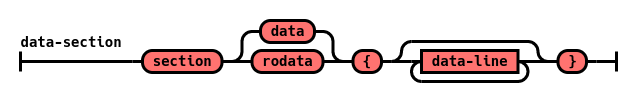
\includegraphics{nstar/sections/data-1}
  }\\
  \scalebox{.5}{
    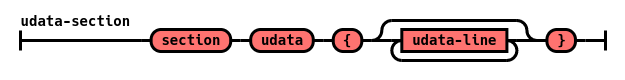
\includegraphics{nstar/sections/data-2}
  }\\
  \scalebox{.5}{
    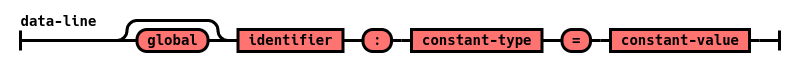
\includegraphics{nstar/sections/data-3}
  }\\
  \scalebox{.5}{
    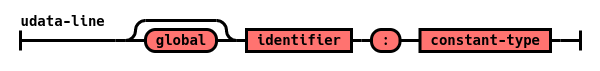
\includegraphics{nstar/sections/data-4}
  }

  \caption{Grammar for the \texttt{data}, \texttt{rodata} and \texttt{udata} sections.}
  \label{fig:nstar-common-sections-data-grammar}
\end{figure}

\noindent Note that, while the grammar allows labels in the \texttt{data} section to be pointers to context types, this cannot be typed because there is no such constant value referencing a code-space address.

While the \texttt{data} and \texttt{rodata} sections contain initialised values (that is, hardcoded bytes in the executable), the \texttt{udata} section does not contain any byte (it should be only $0$s, to reserve space for each entry).

Each label can also be marked with a \texttt{global} qualifier, which acts the same as in the \texttt{code} section.

\subsection{The \texttt{extern} sections}\label{subsec:nstar-common-sections-extern}

The \texttt{extern} sections contain information related to static and dynamic imports.
They come in 2 flavors: function imports or data imports.

\subsubsection{The \texttt{extern.code} section}\label{subsubsec:nstar-common-sections-extern-code}

The \texttt{extern.code} section indicates that there are functions which, despite not being in the source file, should be accessible with the given context.
Static imports are resolved during linking, preventing from using undefined function symbols at runtime, while dynamic imports are resolved at runtime by the dynamic linker.
The two types of imports are indicated from the absence (or presence) of the \texttt{dyn} qualifier when importing.
The grammar showing this is given in figure~\ref{fig:nstar-common-sections-extern-code-grammar}.

\begin{figure}[htb]
  \centering
  \scalebox{.47}{
    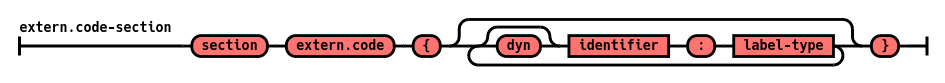
\includegraphics{nstar/sections/externcode-grammar}
  }

  \caption{Grammar for the \texttt{extern.code} file section.}
  \label{fig:nstar-common-sections-extern-code-grammar}
\end{figure}

\subsubsection{The \texttt{extern.data} and \texttt{extern.rodata} sections}\label{subsubsec:nstar-common-sections-extern-data}

The \texttt{extern.data} and \texttt{extern.rodata} sections are used to import data addresses into the current scope.
While it is possible to dynamically import a data address, it shouldn't really be useful (unless in specific cases like \texttt{static} variables).
Same as for the \texttt{extern.code} section, the import type (dynamic or static) is given depending on the absence (or presence) of the \texttt{dyn} qualifier.
The grammar for this section is given in Figure~\ref{fig:nstar-common-sections-extern-data-grammar}.

\begin{figure}[htb]
  \centering
  \scalebox{.45}{
    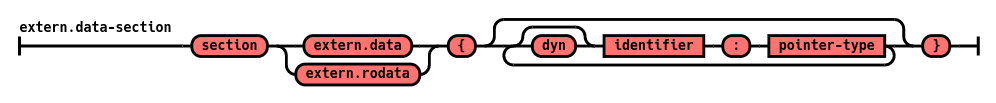
\includegraphics{nstar/sections/externdata-grammar}
  }

  \caption{Grammar for the \texttt{extern.data} and \texttt{extern.rodata} sections.}
  \label{fig:nstar-common-sections-extern-data-grammar}
\end{figure}

\section{Constant values}\label{sec:nstar-common-constvalue}

Constant values are some kind of values that can be used in the \texttt{data} and \texttt{rodata} sections\footnote{See Section~\ref{subsec:nstar-common-sections-data}~``\nameref{subsec:nstar-common-sections-data}''.}.
They come in 3 flavors: integers, characters and arrays.
Their grammar is given in Figure~\ref{fig:nstar-common-constvalue-grammar} and the type inference rules are given in Figure~\ref{fig:nstar-common-constvalue-typerules}.

\begin{figure}[htb]
  \centering
  \scalebox{.5}{
    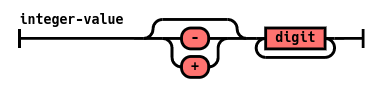
\includegraphics{nstar/constants/integer-grammar}
  }
  \\
  \scalebox{.5}{
    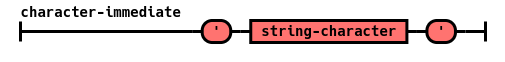
\includegraphics{nstar/constants/character-grammar}
  }
  \\
  \scalebox{.5}{
    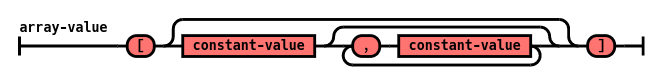
\includegraphics{nstar/constants/array-grammar}
  }

  \caption{Grammar for constant values.}
  \label{fig:nstar-common-constvalue-grammar}
\end{figure}

\begin{figure}[htb]
  \centering

  \begin{prooftree}
    \hypo{$d is a signed integer constant$}
    \hypo{$t $\in\{$s8, s16, s32, s64$\}}
    \infer2{\Gamma\vdash^T_{data}$ d : t$}
  \end{prooftree}
  \\\vspace{\baselineskip}
  \begin{prooftree}
    \hypo{$d is an unsigned integer constant$}
    \hypo{$t $\in\{$u8, u16, u32, u64$\}}
    \infer2{\Gamma\vdash^T_{data}$ d : t$}
  \end{prooftree}
  \\\vspace{\baselineskip}
  \begin{prooftree}
    \hypo{$c is a character constant$}
    \infer1{\Gamma\vdash^T_{data}$ c : char$}
  \end{prooftree}
  \\\vspace{\baselineskip}
  \begin{prooftree}
    \hypo{$n : $\mathbb{N}}
    \hypo{\Gamma\vdash^K$ t : Tn$}
    \hypo{\Gamma\vdash^T_{data}$ c$_1$, c$_2$, \ldots, c$_n$ : t$}
    \infer3{\Gamma\vdash^T_{data}$ [c$_1$, c$_2$, \ldots, c$_n$] : *t$}
  \end{prooftree}

  \caption{Type inference rules for constant values.}
  \label{fig:nstar-common-constvalue-typerules}
\end{figure}

\section{Restrictions applied to branching}\label{sec:nstar-common-bs-restrictions}

Branching ((un-)\ conditional jumps, calls, etc) is restricted in N* in order to prevent stack leaks, unknown caller address return or even missing return values.
It also is restricted not to integrate some sort of scoping, which would add some (mostly useless) complexity when using/generating N*.

\subsection{Returning to a known code-space address}\label{subsec:nstar-common-bs-restrictions-ret}

N* offers what we call ``continuations'', which are a mean of easily controlling the instruction control flow of the program.
Thanks to that, this is actually easy to check whether we would be returning to some valid piece of code: the continuation part of th context must be bound to something of the form $\forall().ctx$.
When anything else is in the continuation (in fact, it cannot be, because we do not allow overwriting the continuation --- which can be worked around by moving the continuation somewhere else before), it is strictly impossible to either \texttt{call} or \texttt{jmp} to a label, or \texttt{ret} from a piece of code, which would yield a very nasty undefined behavior at runtime in mainstream assembly languages.

\subsection{Missing return values (a.k.a.\ registers not bound before return)}\label{subsec:nstar-common-bs-restrictions-unboundregs}

Along with checking that we are returning to a valid code-space address, we can also, thanks to context types, determine if returning from a function preserves the value in registers, and if after returning we have access to return values of a function.
Consider the example given in Listing~\ref{lst:nstar-common-bs-returnvalues}.

When \texttt{ret}urning from the \texttt{example} ``function'', we give access to the values of type \texttt{u64} in the \texttt{\%r0} and \texttt{\%r3} registers.
Note that if either of those registers were not bound before (not given as parameters, or bound using \texttt{mv}), type-checking \textit{must} fail to prevent undefined behavior when later accessing the ``value'' in either register.
We can easily see that the return context contains \texttt{\%r0: u64} and \texttt{\%r3: u64}, which means that both registers must have been bound before, and are accessible for reading later on, after the \texttt{call} that went until here.
This gives a safe way of using return values, and guaranteeing that there are indeed return values stored in the target registers.

\begin{listing}[htb]
  \centering
  \begin{minipage}{0.90\textwidth}
    \begin{minted}[]{\nstarlexer}
    example: forall(s: Ts, e: Tc).{ %r5: forall().{ %r0: u64, %r3: u64 | s -> e } | s -> %r5 }
      mov 0, %r0
      mov 5, %r3
      ret
    \end{minted}
  \end{minipage}
  \caption{An example of returning multiple values from a simple function.}
  \label{lst:nstar-common-bs-returnvalues}
\end{listing}

\section{Unsafe operations}\label{sec:nstar-common-unsafe}

Unsafe operations are operations (sequence of zero or more instructions) whose safety cannot be determined from the current context, or whose evaluation cannot be determined as not UB-provoking (that is, the evaluation may put the application in an unknown state).
Those kind of operations are essential to low-level programming, but we want to put an emphasis on them by separating them from the rest of the normal and safe operations using \texttt{unsafe} blocks.

\subsection{Dereferencing literal addresses}\label{subsec:nstar-common-unsafe-derefliteraladdr}

Sometimes, one needs to be able to read from/write to literal addresses, such as \texttt{0xB8000} in kernel development (this is the console text buffer beginning address, used to output text to the basic 80×25 console).
However, because you cannot guarantee that 1- the memory address exists on every machine the program is supposed to run on and 2- there always are some reconstitutable pieces of data of the specified type at the given address, those two operations are considered unsafe.
Be aware that, despite not being restricted, trying to write to a protected memory address yields an undefined behavior.
Also, if used, the code is no-longer considered platform-independendant\footnote{Platform independant code (PIC for short) is a type of code which should be runnable on all machines, no matter their specifications.}.

\subsection{Pointer offsetting}\label{subsec:nstar-common-unsafe-ptroffset}

Stack pointers, because of their type, can be safely offset to point to a valid piece of data.
However, ``normal'' pointers (for example \texttt{*u64}) cannot be safely offset.
While a stack pointers describes the entire structure of the stack (or at least a piece of it), a regular pointer only describes the piece of data it points to.

This is a common idiom in C to use pointers to represent arrays in a contiguous memory (so an array of 6 integers would basically be a $6 * sizeof(int)$ bytes wide chunk of memory, where each index points to a different integer).
\texttt{Vec<T>} in Rust, \texttt{std::vector<T>} in C++, \texttt{ArrayList<T>} in Java, and many other vector types are also implemented in terms of a pointer to a chunk of memory, but with an added container size, allowing to safely access elements of the vector without going out of bounds.
But in Rust, we still need to have some \texttt{unsafe} blocks in your code, in order to use the container.

There is the same problem in N*.
Because there is no built-in array type, we have to rely on pointers to be able to achieve such thing, therefore needing a way to offset a pointer to access the various elements in the array.
It would also be really hard to manipulate plain array types (because, for example, of the size to store with the type).
As offsetting a pointer can lead to an invalid address dereferencing (or at least dereferencing an address which doesn't belong to the application memory, i.e.\ allocated by another process), it is considered an unsafe operation and therefore needs to be wrapped in an \texttt{unsafe} block.

\subsection{Pointer offsetting using a register}\label{subsec:nstar-common-unsafe-ptroffsetreg}

Offsetting a stack pointer or a structure pointer is considered a safe operation because it is possible to guarantee at compile-time that the offset is correct and points to valid data, unless the offset is a register.
Because of this, offsetting any pointer using a register (e.g. \texttt{\%r1(\$0 : u64)}) is considered an unsafe operation and should be surrounded by an \texttt{unsafe} block, no matter the instruction used (\texttt{mov}, \texttt{push}, \texttt{pop}, \ldots).

\chapter{Instruction set}\label{chap:nstar-instructionset}

\section{\texttt{mv}}\label{sec:nstar-instructionset-mv}

The \texttt{mv} instruction moves a value (immediate value or stored in a register) into a register.
Grammar is given in Figure~\ref{fig:nstar-instructionset-mv-grammar}.
Type inference rules are given in Figure~\ref{fig:nstar-instructionset-mv-typerules}.

\begin{figure}[H]
  \centering
  \scalebox{.5}{
    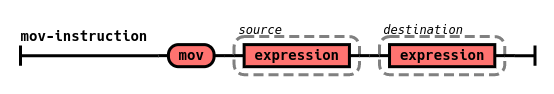
\includegraphics{nstar/instructions/mov-grammar}
  }
  \caption{Grammar of the \texttt{mv} instruction.}
  \label{fig:nstar-instructionset-mv-grammar}
\end{figure}

\begin{figure}[H]
  \centering

  \begin{prooftree}
    \hypo{$r, d are registers$}
    \hypo{\Xi;\Gamma;\chi;\sigma;\epsilon\vdash^T_{code}$ r : $\forall$().ctx$}
    \infer2[move cont from register to register]{\Xi;\Gamma;\chi;\sigma;$ r $\vdash^I$ mv r, d $\dashv\chi,$ d : $\forall$().ctx$;\sigma;$ d$}
  \end{prooftree}
  \\\vspace{\baselineskip}
  \begin{prooftree}
    \hypo{$r is a register$}
    \hypo{$n $\leq 8}
    \hypo{\Gamma\vdash^K$ t : Tn$}
    \hypo{\Xi;\Gamma;\chi;\sigma;\epsilon\vdash^T_{code}$ e : t$}
    \infer4[move value to register]{\Xi;\Gamma;\chi;\sigma;\epsilon\vdash^I$ mv e, r $\dashv\chi\setminus$r, r : t$;\sigma;\epsilon}
  \end{prooftree}

  \caption{Type inference rules for the \texttt{mv} instruction.}
  \label{fig:nstar-instructionset-mv-typerules}
\end{figure}

\section{\texttt{sst}}\label{sec:nstar-instructionset-sst}

The \texttt{sst} instruction stores a value at the given index on the stack.
Grammar and inference rules are given in Figure~\ref{fig:nstar-instructionset-sst-grammar} and Figure~\ref{fig:nstar-instructionset-sst-typerules}.

\begin{figure}[H]
  \centering

  \scalebox{.5}{
    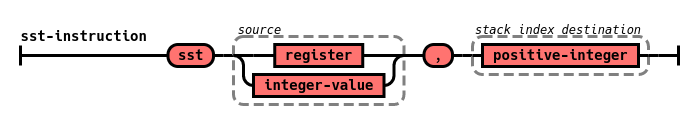
\includegraphics{nstar/instructions/sst-grammar}
  }

  \caption{Grammar for the \texttt{sst} instruction.}
  \label{fig:nstar-instructionset-sst-grammar}
\end{figure}

\begin{figure}[H]
  \centering

  \begin{prooftree}
    \hypo{$r is a register$}
    \hypo{$n $\in\mathbb{N}}
    \hypo{\hat{\sigma}=$ t$_0$::t$_1$::\ldots::t$_p$::s$}
    \infer[no rule, rule margin=1.0ex]3{\Gamma\vdash^K$ t : T8\hspace{1.5em}$%
                                        $n $\leq$ p$}
    \infer[no rule, rule margin=1.0ex]1{\hat{\sigma}^\prime=\hat{\sigma}[\forall$().ctx$\setminus$t$_n]$\hspace{1.5em}$%
                                        \Xi;\Gamma;\chi;\hat{\sigma};\epsilon\vdash^T_{code}$ r : $\forall$().ctx\hspace{1.5em}$%
                                        $t$_n\sim$ t$}
    \infer1[store cont from register to stack]{\Xi;\Gamma;\chi;\hat{\sigma};$ r $\vdash^I$ sst r, n $\dashv\chi;\hat{\sigma}^\prime;$ n$}
  \end{prooftree}
  \\\vspace{\baselineskip}
  \begin{prooftree}
    \hypo{$n $\in\mathbb{N}}
    \hypo{\hat{\sigma}=$ t$_0$::t$_1$::\ldots::t$_p$::s$}
    \hypo{$n $\leq$ p$}
    \hypo{\Xi;\Gamma;\chi;\hat{\sigma};\epsilon\vdash^T_{code}$ e : t$_n}
    \infer4[store value in stack]{\Xi;\Gamma;\chi;\hat{\sigma};\epsilon\vdash^I$ sst e, n $\dashv\chi;\hat{\sigma};\epsilon}
  \end{prooftree}


  \caption{Type inference rules for the \texttt{sst} instruction.}
  \label{fig:nstar-instructionset-sst-typerules}
\end{figure}

\section{\texttt{sld}}\label{sec:nstar-instructionset-sld}

The \texttt{sld} instruction stores the value at the given index on the stack in a register.
Grammar and inference rules are given in Figure~\ref{fig:nstar-instructionset-sld-grammar} and Figure~\ref{fig:nstar-instructionset-sld-typerules}.

\begin{figure}[H]
  \centering

  \scalebox{.5}{
    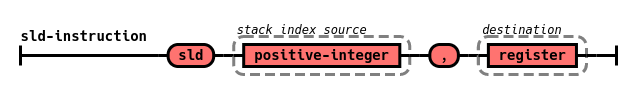
\includegraphics{nstar/instructions/sld-grammar}
  }

  \caption{Grammar for the \texttt{sld} instruction.}
  \label{fig:nstar-instructionset-sld-grammar}
\end{figure}

\begin{figure}[H]
  \centering

  \begin{prooftree}
    \hypo{$r is a register$}
    \hypo{$n $\in\mathbb{N}}
    \hypo{$n $\leq$ p$}
    \infer[no rule, rule margin=1.0ex]3{\hat{\sigma}=$ t$_0$::t$_1$::\ldots::t$_p$::s\hspace{1.5em}$%
                                        $t$_n\sim\forall$().ctx$}
    \infer1[load cont from stack in register]{\Xi;\Gamma;\chi;\hat{\sigma};$ n $\vdash^I$ sld n, r $\dashv\chi,$ r : t$_n;\hat{\sigma};$ r$}
  \end{prooftree}
  \\\vspace{\baselineskip}
  \begin{prooftree}
    \hypo{$r is a register$}
    \hypo{$n, k $\in\mathbb{N}}
    \infer[no rule, rule margin=1.0ex]2{$n $\leq$ p\hspace{1.5em}$%
                                        $k $\leq8$\hspace{1.5em}$%
                                        \hat{\sigma}=$ t$_0$::t$_1$::\ldots::t$_p$::s\hspace{1.5em}$%
                                        \Gamma\vdash^K$ t$_n$ : Tk$}
    \infer1[load value from stack]{\Xi;\Gamma;\chi;\hat{\sigma};\epsilon\vdash^I$ sld n, r $\dashv\chi,$ r : t$_n;\hat{\sigma};\epsilon}
  \end{prooftree}

  \caption{Type inference rules for the \texttt{sld} instruction.}
  \label{fig:nstar-instructionset-sld-typerules}
\end{figure}

\section{\texttt{st}}\label{sec:nstar-instructionset-st}

The \texttt{st} instruction stores a value into a memory area denoted by pointer offset.
The grammar and inference rules are given in Figure~\ref{fig:nstar-instructionset-st-grammar} and Figure~\ref{fig:nstar-instructionset-st-typerules}.

\begin{figure}[H]
  \centering

  \scalebox{.5}{
    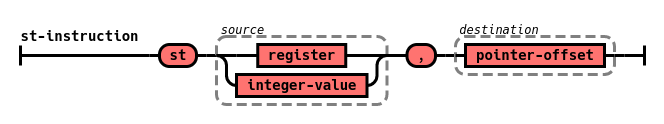
\includegraphics{nstar/instructions/st-grammar}
  }

  \caption{Grammar for the \texttt{st} instruction.}
  \label{fig:nstar-instructionset-st-grammar}
\end{figure}

\begin{figure}[H]
  \centering

  \begin{prooftree}
    \hypo{\Xi;\Gamma;\chi;\sigma;\epsilon\vdash^T_{code}$ e : t$}
    \hypo{$e $\neq\epsilon}
    \hypo{\Xi;\Gamma;\chi;\sigma;\epsilon\vdash^T_{code}$ o(p) : *t$}
    \infer3[store value in pointer byte offset]{\Xi;\Gamma;\chi;\sigma;\epsilon\vdash^I$ st e, o(p) $\dashv\chi;\sigma;\epsilon}
  \end{prooftree}
  \\\vspace{\baselineskip}
  \begin{prooftree}
    \hypo{\Xi;\Gamma;\chi;\sigma;\epsilon\vdash^T_{code}$ e : t$}
    \hypo{$e $\neq\epsilon}
    \hypo{\Xi;\Gamma;\chi;\sigma;\epsilon\vdash^T_{code}$ p[o] : *t$}
    \infer3[store value in pointer base offset]{\Xi;\Gamma;\chi;\sigma;\epsilon\vdash^I$ st e, p[o] $\dashv\chi;\sigma;\epsilon}
  \end{prooftree}

  \caption{Type inference rules for the \texttt{st} instruction.}
  \label{fig:nstar-instructionset-st-typerules}
\end{figure}

\section{\texttt{ld}}\label{sec:nstar-instructionset-ld}

The \texttt{ld} instruction loads a value from a memory area into a register.
Grammar and inference rules are given in Figure~\ref{fig:nstar-instructionset-ld-grammar} and Figure~\ref{fig:nstar-instructionset-ld-typerules}.

\begin{figure}[H]
  \centering

  \scalebox{.5}{
    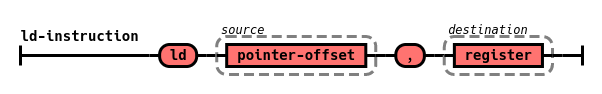
\includegraphics{nstar/instructions/ld-grammar}
  }

  \caption{Grammar for the \texttt{ld} instruction.}
  \label{fig:nstar-instructionset-ld-grammar}
\end{figure}

\begin{figure}[H]
  \centering

  \begin{prooftree}
    \hypo{$r is a register$}
    \hypo{$r $\neq\epsilon}
    \hypo{\Xi;\Gamma;\chi;\sigma;\epsilon\vdash^T_{code}$ o(p) : *t$}
    \infer3[load value from pointer byte offset]{\Xi;\Gamma;\chi;\sigma;\epsilon\vdash^I$ ld o(p), r $\dashv\chi,$ r : t$;\sigma;\epsilon}
  \end{prooftree}
  \\\vspace{\baselineskip}
  \begin{prooftree}
    \hypo{$r is a register$}
    \hypo{$r $\neq\epsilon}
    \hypo{\Xi;\Gamma;\chi;\sigma;\epsilon\vdash^T_{code}$ p[o] : *t$}
    \infer3[load value from pointer base offset]{\Xi;\Gamma;\chi;\sigma;\epsilon\vdash^I$ ld p[o], r $\dashv\chi,$ r : t$;\sigma;\epsilon}
  \end{prooftree}

  \caption{Type inference rules for the \texttt{ld} instruction.}
  \label{fig:nstar-instructionset-ld-typerules}
\end{figure}

\section{\texttt{jmp}}\label{sec:nstar-instructionset-jmp}

The \texttt{jmp} instruction moves the instruction pointer to the given code-space address (specified using a label).
Grammar and inference rules are respectively given in Figure~\ref{fig:nstar-instructionset-jmp-grammar} and Figure~\ref{fig:nstar-instructionset-jmp-typerules}.

\begin{figure}[H]
  \centering

  \scalebox{.5}{
    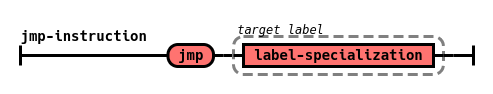
\includegraphics{nstar/instructions/jmp-grammar}
  }

  \caption{Grammar of the \texttt{jmp} instruction.}
  \label{fig:nstar-instructionset-jmp-grammar}
\end{figure}

\begin{figure}[H]
  \centering

  \begin{prooftree}
    \hypo{\Xi;\Gamma;\chi;\sigma;\epsilon\vdash^T_{code}$ l<$\vec{v}$> : $\forall$().\{ $\chi^\prime$ | $\sigma\to\epsilon$ \}$}
    \hypo{\chi\sim\chi^\prime}
    \infer2[jump to label]{\Xi;\Gamma;\chi;\sigma;\epsilon\vdash^I$ jmp l<$\vec{v}$> $\dashv\chi;\sigma;\epsilon}
  \end{prooftree}

  \caption{Type inference rules for the \texttt{jmp} instruction.}
  \label{fig:nstar-instructionset-jmp-typerules}
\end{figure}

The result context is exactly the same as the input context, but this is not a problem because jumps can only be used at the end of blocks, where the result context does not matter at all.

\section{\texttt{call}}\label{sec:nstar-instructionset-call}

The \texttt{call} instruction simply jumps to the target address (specified using a label).
Grammar and inference rules are given in Figure~\ref{fig:nstar-instructionset-call-grammar} and Figure~\ref{fig:nstar-instructionset-call-typerules}.

\begin{figure}[H]
  \centering

  \scalebox{.5}{
    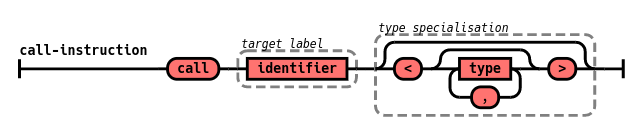
\includegraphics{nstar/instructions/call-grammar}
  }

  \caption{Grammar of the \texttt{call} instruction.}
  \label{fig:nstar-instructionset-call-grammar}
\end{figure}

\begin{figure}[H]
  \centering

  \begin{prooftree}
    \hypo{$r is a register$}
    \hypo{\Xi;\Gamma;\chi;\sigma;\epsilon\vdash^T_{code}$ l<$\vec{v}$> : $\forall$().\{ $\hat{\chi}$ | $\sigma\to$ r \}$}
    \infer[no rule, rule margin=1.0ex]2{\Xi;\Gamma;\hat{\chi};\hat{\sigma};$ r $\vdash^T_{code}$ r : $\forall$().\{ $\chi^\prime$ | $\sigma^\prime\to\epsilon^\prime$ \}\hspace{1.5em}$%
                                        \chi\sim\hat{\chi}}

    \infer1[function call]{\Xi;\Gamma;\chi;\sigma;\epsilon\vdash^I$ call l<$\vec{v}$> $\dashv\chi;\sigma;\epsilon}
  \end{prooftree}
  \\\vspace{\baselineskip}
  \begin{prooftree}
    \hypo{$n $\in\mathbb{N}}
    \hypo{$n $\leq$ p$}
    \hypo{\Xi;\Gamma;\chi;\sigma;\epsilon\vdash^T_{code}$ l<$\vec{v}$> : $\forall$().\{ $\hat{\chi}$ | $\sigma\to$ n \}$}
    \infer[no rule, rule margin=1.0ex]3{$t$_n\sim\forall$().\{ $\chi^\prime$ | $\sigma^\prime\to\epsilon^\prime$ \}\hspace{1.5em}$%
                                        \chi\sim\hat{\chi}$\hspace{1.5em}$%
                                        \sigma=$ t$_0$::t$_1$::\ldots::t$_p$::s$}
    \infer1[function call]{\Xi;\Gamma;\chi;\sigma;\epsilon\vdash^I$ call l<$\vec{v}$> $\dashv\chi;\sigma;\epsilon}
  \end{prooftree}

  \caption{Type inference rules for the \texttt{call} instruction.}
  \label{fig:nstar-instructionset-call-typerules}
\end{figure}

\section{\texttt{ret}}\label{sec:nstar-instructionset-ret}

The \texttt{ret} instruction moves the instruction pointer to the address on top of the stack, and pops it from the stack.
It is essentially equivalent to doing \texttt{pop \%ip} at runtime.
Grammar is given in Figure~\ref{fig:nstar-instructionset-ret-grammar} and type inference rules are given in Figure~\ref{fig:nstar-instructionset-ret-typerules}.

\begin{figure}[H]
  \centering

  \scalebox{.5}{
    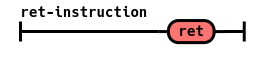
\includegraphics{nstar/instructions/ret-grammar}
  }

  \caption{Grammar for the \texttt{ret} instruction.}
  \label{fig:nstar-instructionset-ret-grammar}
\end{figure}

\begin{figure}[H]
  \centering

  \begin{prooftree}
    \hypo{$r is a register$}
    \hypo{\Xi;\Gamma;\chi;\sigma;$ r $\vdash^T_{code}$ r : $\forall$().\{ $\chi^\prime$ | $\sigma\to\epsilon$ \}$}
    \hypo{\chi\sim\chi^\prime}
    \infer3[return to caller in register]{\Xi;\Gamma;\chi;\sigma;$ r $\vdash^I$ ret $\dashv\chi;\sigma;$ r$}
  \end{prooftree}

  \caption{Type inference rules for the \texttt{ret} instruction.}
  \label{fig:nstar-instructionset-ret-typerules}
\end{figure}

\section{\texttt{nop}}\label{sec:nstar-instructionset-nop}

The \texttt{nop} instruction does absolutely nothing else than skipping a CPU cycle.
Grammar and type inference rules are respectively given in Figure~\ref{fig:nstar-instructionset-nop-grammar} and Figure~\ref{fig:nstar-instructionset-nop-typerules}.

\begin{figure}[H]
  \centering

  \scalebox{.5}{
    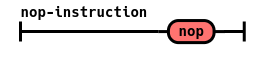
\includegraphics{nstar/instructions/nop-grammar}
  }

  \caption{Grammar for the \texttt{nop} instruction.}
  \label{fig:nstar-instructionset-nop-grammar}
\end{figure}

\begin{figure}[H]
  \centering

  \begin{prooftree}
    \infer0{\Xi;\Gamma;\chi;\sigma;\epsilon\vdash^I$ nop $\dashv\chi;\sigma;\epsilon}
  \end{prooftree}

  \caption{Type inference rules for the \texttt{nop} instruction.}
  \label{fig:nstar-instructionset-nop-typerules}
\end{figure}

\section{\texttt{salloc}}\label{sec:nstar-instructionset-salloc}

The \texttt{salloc} instructions allocates some space on top of the stack for some data of the given type.
Grammar and type inference rules are given in Figure~\ref{fig:nstar-instructionset-salloc-grammar} and Figure~\ref{fig:nstar-instructionset-salloc-typerules}.

\begin{figure}[H]
  \centering

  \scalebox{.5}{
    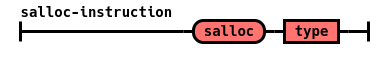
\includegraphics{nstar/instructions/salloc-grammar}
  }

  \caption{Grammar for the \texttt{salloc} instruction.}
  \label{fig:nstar-instructionset-salloc-grammar}
\end{figure}

\begin{figure}[H]
  \centering

  \begin{prooftree}
    \hypo{$n, m $\in\mathbb{N}}
    \hypo{\Gamma\vdash^K$ t : Tm$}
    \hypo{\sigma^\prime=$ t::$\sigma}
    \infer3[\texttt{salloc} with stack continuation]{\Xi;\Gamma;\chi;\sigma;$ n $\vdash^I$ salloc t $\dashv\chi;\sigma^\prime;$ n$+1}
  \end{prooftree}
  \\\vspace{\baselineskip}
  \begin{prooftree}
    \hypo{$m $\in\mathbb{N}}
    \hypo{\Gamma\vdash^K$ t : Tm$}
    \hypo{\sigma^\prime=$ t::$\sigma}
    \infer3{\Xi;\Gamma;\chi;\sigma;\epsilon\vdash^I$ salloc t $\dashv\chi;\sigma^\prime;\epsilon}
  \end{prooftree}

  \caption{Type inference rules for the \texttt{salloc} instruction.}
  \label{fig:nstar-instructionset-salloc-typerules}
\end{figure}

\section{\texttt{sfree}}\label{sec:nstar-instructionset-sfree}

The \texttt{sfree} instruction frees the top-most stack cell.
Grammar and type inference rules are respectively given in Figure~\ref{fig:nstar-instructionset-sfree-grammar} and Figure~\ref{fig:nstar-instructionset-sfree-typerules}.

\begin{figure}[H]
  \centering

  \scalebox{.5}{
    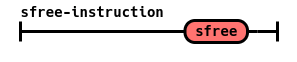
\includegraphics{nstar/instructions/sfree-grammar}
  }

  \caption{Grammar for the \texttt{sfree} instruction.}
  \label{fig:nstar-instructionset-sfree-grammar}
\end{figure}

\begin{figure}[H]
  \centering

  \begin{prooftree}
    \hypo{$n $\geq 1}
    \hypo{$n $\leq$ p$}
    \hypo{\sigma=$ t$_0$::t$_1$::\ldots::t$_p$::s$}
    \hypo{\sigma^\prime=$ t$_1$::\ldots::t$_p$::s$}
    \infer4[\texttt{sfree} with stack continuation]{\Xi;\Gamma;\chi;\sigma;$ n $\vdash^I$ sfree $\dashv\chi;\sigma^\prime;$ n$-1}
  \end{prooftree}
  \\\vspace{\baselineskip}
  \begin{prooftree}
    \hypo{\sigma=$ t$_0$::t$_1$::\ldots::t$_p$::s$}
    \hypo{\sigma^\prime=$ t$_1$::\ldots::t$_p$::s$}
    \infer2{\Xi;\Gamma;\chi;\sigma;\epsilon\vdash^I$ sfree $\dashv\chi;\sigma^\prime;\epsilon}
  \end{prooftree}

  \caption{Type inference rules for the \texttt{sfree} instruction.}
  \label{fig:nstar-instructionset-sfree-typerules}
\end{figure}

\chapter{Target-dependent features}\label{chap:nstar-specific}

\section{x86, amd64}\label{sec:nstar-specific-x86amd64}

\subsection{Register mappings}\label{subsec:nstar-specific-x86amd64-registers}

\begin{tabularx}{\textwidth}{Y Y Y}
  \toprule
  N* & x86 & amd64 \\
  \midrule
  r0 & eax & rax \\
  r1 & ecx & rcx \\
  r2 & edx & rdx \\
  r3 & ebx & rbx \\
  r4 & esi & rsi \\
  r5 & edi & rdi \\
  \bottomrule
\end{tabularx}
